\subsection{Namespace Graph}\label{app:ns-detail}

\subsubsection{Containment Decay}

\begin{table}[ht]
\centering
\caption[Containment across granularity levels]{Containment across granularity levels. Namespace-depth rows are computed on all $8{,}436{,}366$ edges of $G_{\mathrm{thm}}$. The top-level directory and file-level rows are computed on the $2{,}506{,}738$ edges whose both endpoints appear in the file-module mapping.\protect\footnotemark}
\label{tab:containment-decay}
\begin{tabular}{llrr}
\toprule
Granularity & Units & Cross-boundary & Containment \\
\midrule
Top-level directory             & $32$          & $51.1\%$ & $48.9\%$ \\
Namespace depth $1$             & $3{,}184$     & $77.8\%$ & $22.2\%$ \\
Namespace depth $2$             & $10{,}097$    & $85.8\%$ & $14.2\%$ \\
File-level                      & $7{,}225$     & $84.4\%$ & $15.6\%$ \\
Namespace depth $\ge 3$         & ${\sim}15$K   & $87.4\%$ & $12.6\%$ \\
\bottomrule
\end{tabular}
\end{table}
\footnotetext{The file-module mapping covers $217{,}647$ of $308{,}129$ declarations; unmapped declarations are primarily Lean core infrastructure residing outside the \texttt{Mathlib/} source tree.}

\begin{figure}[ht]
\centering

\includegraphics[width=0.82\textwidth]{figures/containment_curve.pdf}
\caption{Containment decay curve. Green circles connected by the solid line show containment at namespace depth $k = 1, \ldots, 6$; blue squares mark file-system levels (top-level directory and file module). The gray dashed line marks the same-file baseline from Table~\ref{tab:thm-edge-breakdown} ($9.6\%$). Containment drops steeply from the top-level directory to depth~$1$ and saturates by depth~$3$.}
\label{fig:containment-curve}
\end{figure}

The decay exhibits three regimes.

\paragraph{Discipline-level containment (top-level directory, 48.9\%).} At the coarsest granularity---the $32$ top-level directories (\module{Algebra}, \module{CategoryTheory}, \module{Topology}, etc.)---nearly half of all declaration-level dependencies stay within the same directory. These discipline-level categories, inherited from centuries of mathematical practice, retain genuine organizational force. Yet more than half of all dependencies cross directory boundaries---no discipline is self-contained.

\paragraph{The steepest drop (top-level directory $\to$ depth~$1$, $48.9\% \to 22.2\%$).} The largest single decrease occurs when we move from $32$ directories to $3{,}184$ depth-$1$ namespaces. The steep drop indicates that discipline-level classification exerts substantial constraint on dependencies, but once we enter the interior of a discipline, the namespace boundaries between \ns{Nat} and \ns{Int}---or between \ns{Set} and \ns{Finset}---carry far less force.

\paragraph{Rapid saturation (depth~$2$+, ${\sim}13\%$).} Beyond depth~$2$, containment barely decreases: from $14.2\%$ at depth~$2$ to $12.6\%$ at depth~$6$. Finer naming distinctions add almost no intra-namespace edges. The cross-domain character of mathematical reasoning is fully exposed by the second level of the naming hierarchy.

\paragraph{File-level containment (15.6\%).} The file-module level ($7{,}225$ units) falls between namespace depth~$1$ and depth~$2$ in both granularity and containment. Files offer no containment advantage beyond that of a mid-level namespace.

\subsubsection{Extended Analysis}\label{app:ns-analysis}

\noindent \textit{1. Containment decay as a measure of cognitive boundaries.} \\
The containment decay curve (Figure~\ref{fig:containment-curve}) provides a quantitative measure of a cultural artifact's explanatory power. The disciplinary taxonomy inherited from centuries of mathematical practice---Algebra, Analysis, Topology, Number Theory---``works'' at the broadest scale: nearly half of all declaration-level dependencies stay within the same top-level directory. But this organizing force dissipates rapidly. The steepest single drop ($48.9\% \to 22.2\%$, a loss of $26.7$ percentage points) occurs at the discipline--sub-discipline transition, where the $32$ top-level directories fragment into $3{,}184$ depth-$1$ namespaces. Within a discipline, the boundaries between \ns{Nat} and \ns{Int}, or between \ns{Set} and \ns{Finset}, carry far less constraining power than the boundary between \ns{Algebra} and \ns{Topology}.

The saturation beyond depth~$2$ (${\sim}13\%$) is equally informative: finer naming distinctions add almost no intra-namespace edges. The cross-domain character of mathematical reasoning is fully exposed by the second level of the naming hierarchy. This suggests that the namespace tree is ``informationally shallow''---its first two levels encode most of the dependency structure that human naming captures, and deeper levels serve primarily as disambiguation rather than as semantic boundaries.

The comparison with module-level containment (Table~\ref{tab:module-containment}) is instructive. Module containment at the coarsest level ($97.5\%$ at depth~$1$) is far higher than namespace containment at any level, because module-level edges are import edges between files, which are constrained by the file system's directory structure. Declaration-level edges are unconstrained: a theorem may cite any previously verified result regardless of file location. The gap between $97.5\%$ (module, depth~$1$) and $48.9\%$ (namespace, top-level directory) quantifies the difference between a compiler-enforced organizational constraint and a purely cognitive one.

\medskip
\noindent \textit{2. Structural interpolation between module and declaration levels.} \\
The namespace graph $G_{\mathrm{ns}}^{(2)}$ consistently occupies an intermediate position between the module graph and the declaration graph across all structural metrics. Its modularity ($0.283$) and community--namespace NMI ($0.253$) are both lower than the corresponding declaration-level values, reflecting the coarsening effect of namespace aggregation: merging declarations into namespace nodes absorbs intra-namespace heterogeneity and weakens community boundaries.

This interpolation property makes the namespace graph a useful diagnostic tool. Where the module graph is too coarse (conflating logically unrelated declarations that happen to share a file) and the declaration graph is too fine (with $308{,}129$ nodes that resist visual inspection), the depth-$2$ namespace graph offers a ``medium resolution'' view of Mathlib's dependency structure. The cross-namespace edge density rises from $37.1\%$ at the module level to $50.9\%$ at the declaration level; the namespace graph captures this increase progressively as depth increases, making the transition from contained to entangled visible as a continuous process rather than a binary contrast.

\medskip
\noindent \textit{3. Infrastructure bottleneck and targeted fragility.} \\
The namespace graph is more vulnerable to targeted attack than the declaration graph: $20\%$ targeted removal reduces the giant connected component (GCC) to $20.8\%$ of its original size, versus $46.1\%$ at the declaration level (\S\ref{sec:sa-robustness}). This heightened fragility arises because namespace aggregation concentrates dependencies: a handful of shallow infrastructure namespaces---\ns{Eq}, \ns{OfNat}, \ns{DFunLike}---absorb the dependencies of thousands of declarations, creating namespace-level hubs with extreme in-degree. Removing these hubs at the namespace level is equivalent to removing entire clusters of declarations simultaneously, amplifying the fragmentation effect.

This vulnerability has practical implications. Refactoring or renaming a namespace that serves as an infrastructure bottleneck---for instance, splitting \ns{CategoryTheory} into finer sub-namespaces, or reorganizing the \ns{Algebra} hierarchy---may disrupt a disproportionate fraction of the library's dependency structure. The robustness analysis suggests that such reorganizations should be guided by centrality data: namespaces with high betweenness centrality are structural bridges whose modification carries systemic risk.

\medskip
\noindent \textit{4. Import vs.\ declaration cross-boundary rates.}\label{rem:import-vs-decl-cross} \\
The cross-namespace edge density of $G_{\mathrm{thm}}$ ($50.9\%$; Table~\ref{tab:thm-edge-breakdown}) far exceeds that of $G_{\mathrm{module}}^{-}$ ($37.1\%$; \S\ref{sec:cross-namespace}). This gap reveals that module-level analysis \emph{underestimates} the true extent of mathematical interdependence. Module boundaries bundle cross-namespace theorem dependencies into single intra-directory import edges, creating an illusion of disciplinary containment that dissolves at finer granularity. The namespace graph, by operating at an intermediate resolution, makes this dissolution visible: each step down the depth hierarchy converts contained edges into cross-boundary edges, and the rate of conversion measures the gap between human classification and logical structure.

\subsubsection{Degree Distribution}
\label{sec:ns-degree}

We examine the degree distribution of $G_{\mathrm{ns}}^{(2)}$, the namespace graph at depth~$2$. We choose $k = 2$ because it occupies the sweet spot of the containment decay curve (Table~\ref{tab:containment-decay}): depth~$1$ is too coarse ($3{,}184$ namespaces, comparable to the top-level directory partition), while depth~$3$ and beyond add almost no new cross-boundary structure (containment saturates at ${\sim}13\%$). At depth~$2$, the $10{,}097$ namespaces correspond to familiar mathematical groupings---\ns{Nat.Prime}, \ns{CategoryTheory.Functor}, \ns{MeasureTheory.Measure}---and provide enough nodes for meaningful network analysis. The graph has $332{,}081$ edges (unique namespace pairs), carrying a total weight of $7{,}234{,}844$ declaration-level dependencies.

\begin{table}[ht]
\centering
\caption{Degree statistics for $G_{\mathrm{ns}}^{(2)}$ (unweighted).}
\label{tab:ns-degree-stats}
\begin{tabular}{lrr}
\toprule
& In-degree & Out-degree \\
\midrule
Mean        & $32.9$    & $32.9$ \\
Median      & $1$       & $14$ \\
Std         & $223.2$   & $59.3$ \\
Max         & $9{,}846$ & $3{,}075$ \\
Zero-degree & $3{,}920$ & $6$ \\
\bottomrule
\end{tabular}
\end{table}

The degree distribution is extremely skewed (Table~\ref{tab:ns-degree-stats}). The median in-degree of~$1$ versus a mean of~$33$ reveals a long tail: $3{,}920$ namespaces ($38.8\%$) have zero in-degree---they are referenced by no other namespace---while a handful attract thousands of incoming edges. The top namespaces by in-degree are \ns{\_root\_} ($9{,}846$), \ns{Eq} ($7{,}686$), \ns{OfNat} ($4{,}390$), \ns{Membership} ($3{,}407$), and \ns{Semiring} ($3{,}252$). By out-degree, the leaders are \ns{\_root\_} ($3{,}075$), \ns{MeasureTheory} ($687$), \ns{CategoryTheory} ($656$), and \ns{Polynomial} ($615$).

Power-law fitting (\S\ref{sec:prelim-powerlaw}) yields $\alpha = 1.60$ ($x_{\min} = 4$) for in-degree and $\alpha = 1.90$ ($x_{\min} = 13$) for out-degree. In both cases, a lognormal distribution provides a significantly better fit than a pure power law (likelihood ratio $R = -10.6$ and $R = -289.7$, respectively; $p < 0.01$). This mirrors the pattern observed for $G_{\mathrm{module}}$ (\S\ref{sec:degree-distribution}): heavy-tailed distributions that are not cleanly power-law.

\begin{figure}[ht]
\centering

\includegraphics[width=\textwidth]{figures/ns_degree_distribution.pdf}
\caption{Degree distributions of $G_{\mathrm{ns}}^{(2)}$ on log--log axes. Left: in-degree (\textcolor{blue!60!black}{blue}), with power-law reference (gold dashed, $\alpha = 1.60$, $x_{\min} = 4$). Right: out-degree (\textcolor{red!60!black}{coral}), with power-law reference ($\alpha = 1.90$, $x_{\min} = 13$). Both tails are heavy but better fit by a lognormal than a pure power law. The extreme outlier in the in-degree panel is \ns{\_root\_} ($\deg^{-} = 9{,}846$; see Remark~\ref{rem:root-artifact}).}
\label{fig:ns-degree}
\end{figure}

\noindent\textbf{The \ns{\_root\_} artifact.}
\label{rem:root-artifact}
The namespace \ns{\_root\_} dominates both in-degree and out-degree at depth~$2$. This is an artifact of the truncation rule in Definition~\ref{def:ns-graph}: declarations whose fully qualified names have fewer than three components---including foundational definitions such as \decl{Eq.refl}, \decl{Nat.succ}, and \decl{OfNat.ofNat}---are assigned to \ns{\_root\_}. This namespace is not a coherent conceptual domain; it is a catch-all for the shallow infrastructure of the Lean type system. Its extreme centrality reflects naming-depth convention rather than mathematical importance: the most foundational constructs carry the shortest names. In the analysis that follows, we note where \ns{\_root\_} distorts aggregate statistics.

\paragraph{Cross-level comparison.}
All three levels share heavy-tailed degree distributions in which lognormal fits outperform pure power laws, confirming that the ``few hubs, many low-degree nodes'' pattern is a universal structural feature of the formalized library, independent of analysis granularity. But the differences are equally informative.

\emph{In-degree skewness intensifies with granularity.} At the module level, the in-degree distribution is moderately skewed (median~$2$, mean~$3.1$, max~$167$). At the declaration level, the skewness becomes extreme (median~$1$, mean~$27$, max~$89{,}936$): a handful of language-infrastructure declarations are cited by nearly every proof, while the majority are referenced at most once. The namespace level (median~$1$, mean~$33$, max~$9{,}846$) mirrors this pattern but is distorted by the \ns{\_root\_} artifact (Remark~\ref{rem:root-artifact}).

\emph{Out-degree reveals process constraints.} At the declaration level, out-degree is bounded by the cognitive and logical complexity of a single proof (mean~$27$, max~$522$)---a hard ceiling that no human-written proof exceeds. At the module level, out-degree reflects developer import choices; transitive reduction compresses the maximum from~$315$ to~$70$ and the standard deviation from~$4.12$ to~$1.83$, exposing the development-ergonomic redundancy of umbrella imports (\S\ref{sec:transitive-reduction}). At the declaration level, by contrast, transitive reduction is not meaningful: every premise edge is mechanically extracted from the proof term (Remark~\ref{rem:thm-transitive-reduction}).

This pattern---shared distributional shape but divergent parameters and mechanisms---will recur in the centrality (\S\ref{sec:sa-centrality}) and community (\S\ref{sec:sa-community}) analyses that follow.

\subsubsection{DAG Depth}
\label{sec:ns-dag-depth}

Unlike $G_{\mathrm{module}}$ and $G_{\mathrm{thm}}$, the namespace graph $G_{\mathrm{ns}}^{(2)}$ is \emph{not} a DAG: aggregating declaration-level dependencies to the namespace level creates cycles (e.g., \ns{Nat} $\to$ \ns{Int} $\to$ \ns{Nat}), because declarations in different namespaces can depend on each other bidirectionally (Remark~\ref{rem:ns-cycles}). To recover a layered structure, we condense strongly connected components (SCCs), yielding a DAG of $4{,}080$ super-nodes in $8$ topological layers. The structure is bimodal: layer~$0$ contains $3{,}941$ super-nodes (mostly trivial, single-namespace SCCs that depend on nothing else), while layer~$5$ contains a single super-node---the giant SCC of $5{,}899$ namespaces ($58\%$ of all depth-$2$ namespaces). The intermediate layers ($1$--$4$) hold only $134$ super-nodes that bridge the leaf namespaces to the giant core. Beyond the giant SCC, layers~$6$ and~$7$ contain just $4$ namespaces.

\begin{figure}[ht]
\centering

\includegraphics[width=\textwidth]{figures/ns_dag_structure.pdf}
\caption{Condensed DAG of $G_{\mathrm{ns}}^{(2)}$ by topological layer ($4{,}080$ super-nodes, $8$ layers). Each bar counts the number of super-nodes (SCCs) at that layer. Layer~$0$ holds $3{,}941$ leaf SCCs; layer~$5$ holds a single giant SCC comprising $5{,}899$ namespaces. The shallow, bimodal structure reflects pervasive mutual dependency: most namespaces either sit at the periphery or belong to one densely interconnected core.}
\label{fig:ns-dag-structure}
\end{figure}

\paragraph{Cross-level comparison.} The three DAG depths---$154$ (module), $84$ (declaration), $8$ (namespace, condensed)---reveal a striking inversion. The module graph, organized by human file boundaries, is the \emph{deepest}: its $154$ layers reflect the sequential compilation chain that developers must navigate. The declaration graph, determined by mathematical logic, is shallower: proofs depend on shared infrastructure at moderate depth but rarely form long sequential chains. The namespace graph is nearly flat: at the level of named mathematical concepts, everything depends on everything else, producing dense mutual dependency rather than vertical hierarchy. Depth, in short, is a feature of the production process (file organization) rather than of the mathematical product (logical dependency).

\subsubsection{Centrality}
\label{sec:ns-centrality}

As in \S\ref{sec:centrality} and \S\ref{sec:thm-centrality}, we compute PageRank and betweenness centrality (Definition~\ref{def:pagerank}--\ref{def:betweenness}; $\alpha = 0.85$, weighted; $k = 300$ samples) to identify structurally important namespaces.

\begin{table}[ht]
\centering
\caption{Top~10 namespaces by PageRank and betweenness centrality in $G_{\mathrm{ns}}^{(2)}$.}
\label{tab:ns-centrality}
\small
\begin{tabular}{rlrl}
\toprule
\multicolumn{2}{c}{PageRank} & \multicolumn{2}{c}{Betweenness} \\
\cmidrule(lr){1-2} \cmidrule(lr){3-4}
PR & Namespace & $c_B$ & Namespace \\
\midrule
.247 & \ns{\_root\_}          & .248 & \ns{\_root\_} \\
.035 & \ns{Eq}                & .065 & \ns{And} \\
.017 & \ns{Set}               & .043 & \ns{Eq} \\
.015 & \ns{Iff}               & .036 & \ns{Exists} \\
.014 & \ns{OfNat}             & .031 & \ns{Function} \\
.012 & \ns{Real}              & .030 & \ns{Nat} \\
.012 & \ns{Nat}               & .029 & \ns{CategoryTheory} \\
.012 & \ns{CategoryTheory}    & .019 & \ns{MeasureTheory} \\
.010 & \ns{Preorder}          & .018 & \ns{Set} \\
.008 & \ns{Semiring}          & .017 & \ns{Module} \\
\bottomrule
\end{tabular}
\end{table}

Excluding the \ns{\_root\_} artifact (Remark~\ref{rem:root-artifact}), the two rankings reveal a clear separation (Table~\ref{tab:ns-centrality}). PageRank is dominated by mathematical infrastructure: \ns{Eq}, \ns{Set}, \ns{OfNat}, \ns{Real}, and \ns{Preorder}---the foundational types and structures on which proofs ultimately rest. Betweenness centrality, by contrast, promotes logical connectives and bridging concepts: \ns{And}, \ns{Exists}, and \ns{Function} occupy positions~$2$--$5$ by betweenness but do not appear in the PageRank top~$10$. These namespaces serve as structural bridges: proofs in distant mathematical theories must pass through logical connectives to compose their arguments.

This separation echoes the module-level finding of \S\ref{sec:centrality}, where no single module dominates all three centrality measures, and the declaration-level finding of \S\ref{sec:thm-centrality}, where in-degree, PageRank, and betweenness identify disjoint categories of importance. At the namespace level, the two available measures already diverge sharply, confirming that the multidimensionality of structural importance persists across all three granularities. Figures~\ref{fig:ns-centrality-indeg-pr}--\ref{fig:ns-centrality-betw-pr} shows the pairwise scatter plots.

\begin{figure}[H]
\centering
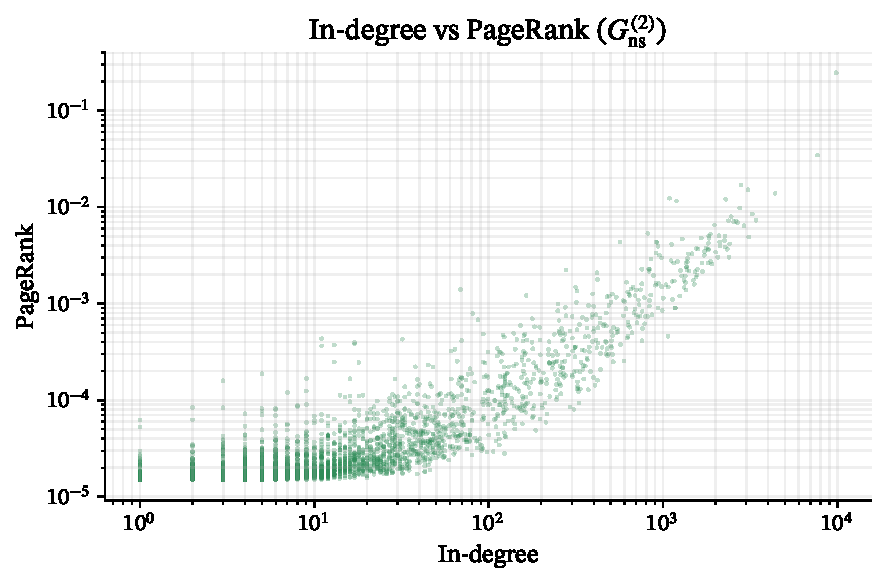
\includegraphics[width=\textwidth]{figures/ns_centrality_indeg_pr.pdf}
\caption{In-degree vs.\ PageRank in $G_{\mathrm{ns}}^{(2)}$. Each point is one namespace. The extreme outlier is \ns{\_root\_} (Remark~\ref{rem:root-artifact}).}
\label{fig:ns-centrality-indeg-pr}
\end{figure}

\begin{figure}[H]
\centering
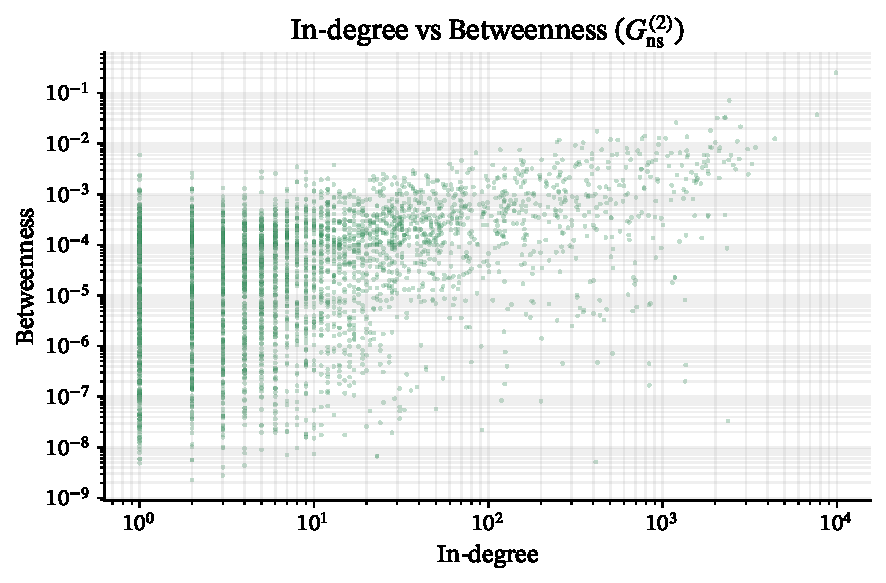
\includegraphics[width=\textwidth]{figures/ns_centrality_indeg_betw.pdf}
\caption{In-degree vs.\ betweenness centrality in $G_{\mathrm{ns}}^{(2)}$. Namespaces with disproportionately high betweenness serve as inter-domain bridges in the namespace dependency graph.}
\label{fig:ns-centrality-indeg-betw}
\end{figure}

\begin{figure}[H]
\centering

\includegraphics[width=\textwidth]{figures/ns_centrality_betw_pr.pdf}
\caption{Betweenness vs.\ PageRank in $G_{\mathrm{ns}}^{(2)}$. Excluding \ns{\_root\_}, the scatter confirms that PageRank and betweenness capture distinct structural roles at the namespace level.}
\label{fig:ns-centrality-betw-pr}
\end{figure}

\subsubsection{Community Structure}
\label{sec:ns-community}

Louvain community detection (\S\ref{sec:prelim-community}) on the undirected, weighted projection of $G_{\mathrm{ns}}^{(2)}$ yields $10$ communities with modularity $Q = 0.283$.

\begin{table}[ht]
\centering
\caption{Top five communities in $G_{\mathrm{ns}}^{(2)}$ by size, with representative namespaces (highest weighted in-degree within each community).}
\label{tab:ns-communities}
\begin{tabular}{rrl}
\toprule
ID & Size & Representative namespaces \\
\midrule
3 & $5{,}096$ & \ns{\_root\_}, \ns{Set}, \ns{Nat} \\
5 & $2{,}227$ & \ns{Semiring}, \ns{NonUnitalNonAssocSemiring}, \ns{DFunLike} \\
4 & $1{,}363$ & \ns{Eq}, \ns{CategoryTheory}, \ns{CategoryTheory.Functor} \\
0 & $1{,}041$ & \ns{Real}, \ns{Zero}, \ns{Field} \\
1 & $360$     & \ns{DivInvMonoid}, \ns{MulOne}, \ns{MulOneClass} \\
\bottomrule
\end{tabular}
\end{table}

The namespace-level community structure differs markedly from the declaration-level structure (\S\ref{sec:thm-community}). At the declaration level, Louvain detection produces $22$ communities with modularity $0.48$ and NMI~$= 0.34$ against the top-level namespace hierarchy. At the namespace level, the number of communities is smaller ($10$ vs.\ $22$), the modularity is lower ($0.283$ vs.\ $0.48$), and the NMI with the top-level directory falls to~$0.253$ (Table~\ref{tab:ns-communities}).

The lower modularity reflects the coarsening inherent in namespace aggregation. When thousands of declarations are collapsed into a single namespace node, the fine-grained community boundaries that Louvain detects at the declaration level are blurred. Edges between namespaces are weighted sums of many declaration-level edges, and the averaging effect smooths out the modular structure that exists at finer granularity. The largest community (ID~$3$, $5{,}096$ nodes) spans half the graph and lacks a coherent mathematical identity: its dominant members (\ns{\_root\_}, \ns{Set}, \ns{Nat}) are foundational constructs used across all disciplines. This contrasts with the declaration-level communities, where the largest communities map onto recognizable mathematical disciplines (\S\ref{sec:thm-community}).

\begin{figure}[H]
\centering
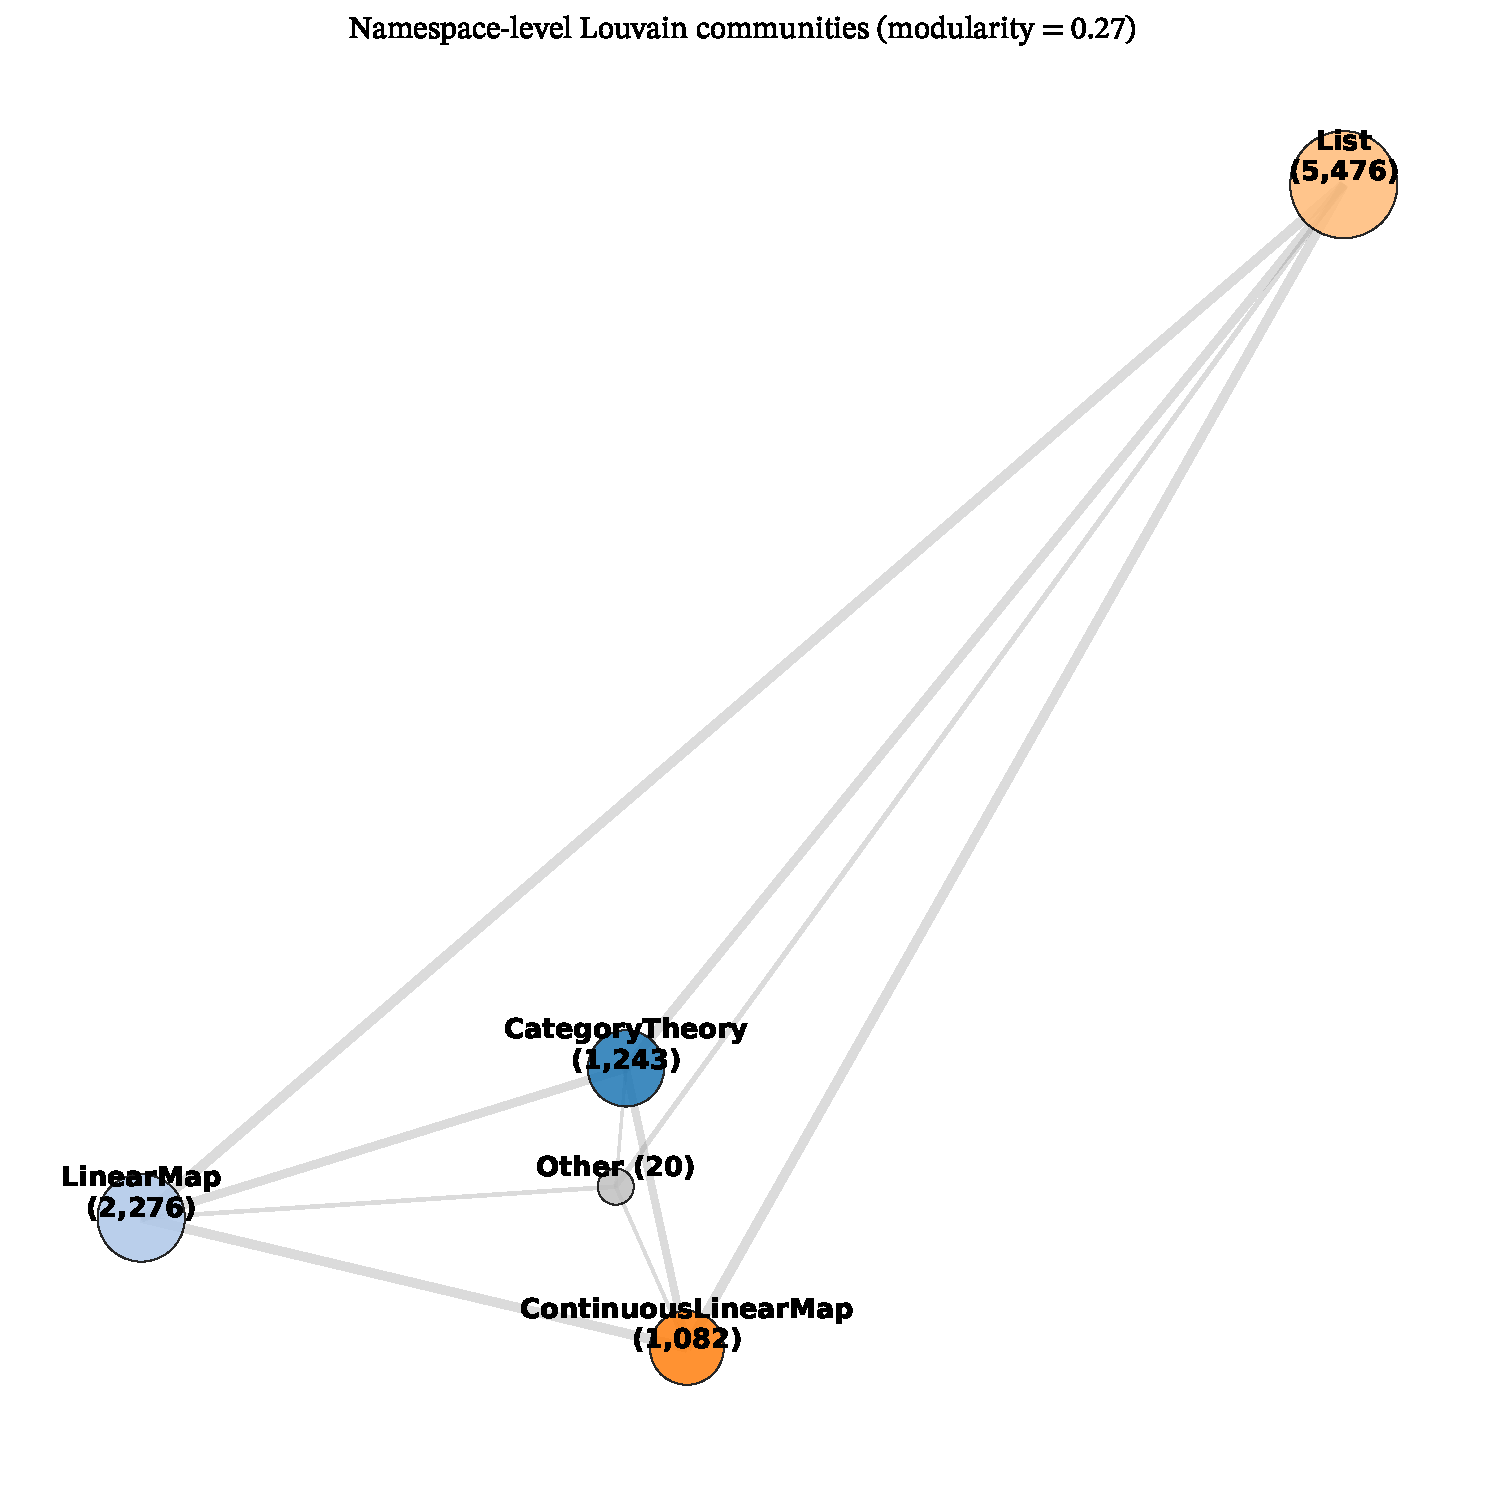
\includegraphics[width=\textwidth]{figures/community_ns_graph.pdf}
\caption{Louvain community aggregation graph of $G_{\mathrm{ns}}^{(2)}$ (modularity~$= 0.28$). Only four communities exceed $0.5\%$ of nodes; the rest are merged into ``Other''. The \ns{List} community absorbs more than half the graph.}
\label{fig:community-ns-graph}
\end{figure}

\begin{figure}[H]
\centering

\includegraphics[width=\textwidth]{figures/community_ns_heatmap.pdf}
\caption{Community$\,\times\,$prefix membership heatmap for $G_{\mathrm{ns}}^{(2)}$ (NMI~$= 0.24$, log scale). Most rows are nearly empty; only three communities show substantive internal structure, confirming that Louvain can barely separate the namespace graph.}
\label{fig:community-ns-heatmap}
\end{figure}

\subsubsection{Robustness}
\label{sec:ns-robustness}

We assess the robustness of $G_{\mathrm{ns}}^{(2)}$ by progressively removing nodes and measuring the fraction of the original graph remaining in the largest weakly connected component (GCC). The original graph has $4$ weakly connected components, with the largest containing $10{,}094$ of $10{,}097$ nodes.

\begin{table}[ht]
\centering
\caption{Robustness of $G_{\mathrm{ns}}^{(2)}$: GCC fraction after random vs.\ targeted (PageRank-ordered) node removal.}
\label{tab:ns-robustness}
\begin{tabular}{rrrr}
\toprule
Removal \% & Random GCC & Targeted GCC & Gap \\
\midrule
$5\%$  & $0.950$ & $0.726$ & $0.223$ \\
$10\%$ & $0.899$ & $0.509$ & $0.391$ \\
$20\%$ & $0.798$ & $0.208$ & $0.590$ \\
$30\%$ & $0.688$ & $0.054$ & $0.634$ \\
$50\%$ & $0.477$ & $0.000$ & $0.477$ \\
\bottomrule
\end{tabular}
\end{table}

\begin{figure}[ht]
\centering
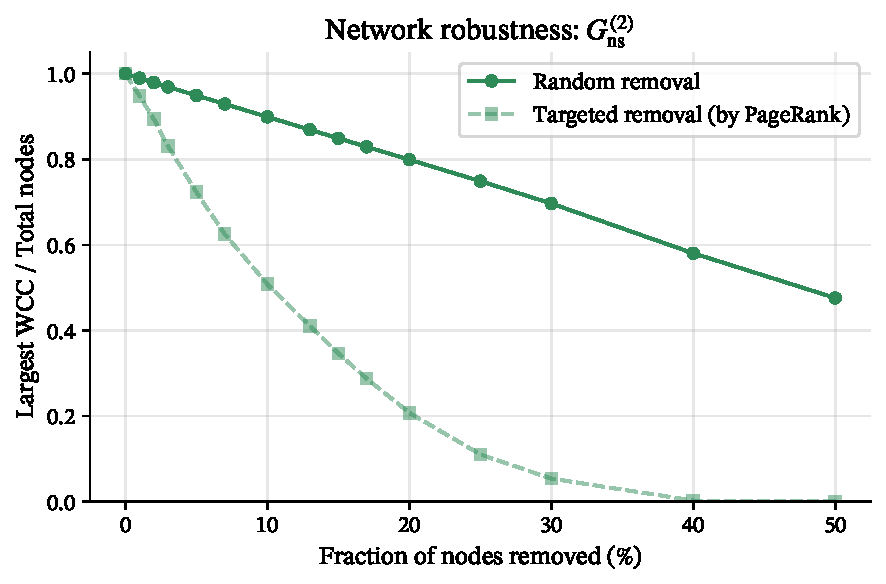
\includegraphics[width=0.85\textwidth]{figures/ns_robustness_curve.pdf}
\caption{Robustness curves for $G_{\mathrm{ns}}^{(2)}$: fraction of nodes in the largest WCC as a function of the fraction removed, under random removal (blue) and targeted removal by PageRank (coral).}
\label{fig:ns-robustness}
\end{figure}

The pattern matches the classic hub-dominated vulnerability signature observed at both the module level (\S\ref{sec:robustness}) and the declaration level (\S\ref{sec:thm-robustness}): high resilience under random failure, extreme fragility under targeted attack (Table~\ref{tab:ns-robustness}, Figure~\ref{fig:ns-robustness}). At $20\%$ targeted removal, the GCC collapses to $20.8\%$ of its original size---more severe than the declaration-level graph, where the same removal fraction leaves $46.1\%$ (\S\ref{sec:thm-robustness}). The namespace graph's greater fragility reflects the concentration of connectivity in the \ns{\_root\_} super-node and a small number of infrastructure namespaces (Remark~\ref{rem:root-artifact}); once these are removed, the remaining mathematical namespaces fragment into isolated clusters with no shared foundation.
